\documentclass{hw}
\usepackage{graphicx}
\usepackage{caption}
\usepackage{subcaption}
\usepackage{float}

\usepackage{xcolor}
\usepackage{enumitem}
\usepackage{listings}
\usepackage{amsmath}% mathtools includes this so this is optional
\usepackage{mathtools}

\def\m{{\textit{m}}}
\def\i{{\textit{i}}}
\def\j{{\textit{j}}}
\def\k{{\textit{k}}}

\newcommand{\hwnum}{4}
\newcommand{\duedate}{December 15, 11:59pm ET}
\renewcommand{\title}{NP Hard, Approximation algorithms}

\newcommand{\io}{\textbf{Code input and output format.} }
\newcommand{\submission}{\textbf{Submission.}}

\setboolean{withsolutions}{false}

\newtheorem{claim}{Claim}

%\usepackage{tikz}
%\usetikzlibrary{positioning}
%\tikzstyle{skipnode} = [rectangle, draw, fill=white, minimum width=1cm, minimum height=0.5cm]
\lstset{
  basicstyle=\ttfamily\scriptsize,    % Use a scriptsize typewriter font
  breaklines=true,               % Break long lines
  frame=single,                  % Frame the code block
  numbers=left,                  % Add line numbers on the left
  numberstyle=\tiny\color{gray}, % Make line numbers small and gray
  keywordstyle=\color{blue},     % Color keywords blue
  commentstyle=\color{green},    % Color comments green
  stringstyle=\color{red},       % Color strings red
}
\begin{document}
\newpage


%%%%%%%%%%%%%%%%%%%%%%%%%%%%%%%%%%%%%%%%%%%%%%%%%%%%%%%%%%%%%%%%%%%%%%%%%%%%%%%%
% Problem 1: Bi-Partite Graphs
\begin{problem}
% https://florian.github.io/count-min-sketch/

Let’s say we want to count the number of times elements appear in a stream of data, $x_1, \dots, x_q$. A simple solution is to maintain a hash table that maps elements to their frequencies.

This approach does not scale: Imagine having an extremely large stream consisting of mostly unique elements. For example, consider network monitoring (either for large network flows or anomalies), large service analytics (e.g. Amazon view/buy counts, Google search popularity), database analytics, etc. Even if we are only interested in the most important ones, this method has huge space requirements. Since we do not know for which items to store counts, our hash table will grow to contain billions of elements.

The Count-Min Sketch, or CMS for short, is a data structure that solves this problem in an approximate way.

\textbf{Approximate Counting with Hashing.}
Given that we only have limited space availability, it would help if we could get away with not storing elements themselves but just their counts. To this end, let’s try to use only an array, with $w$ memory cells, for storing counts as shown below in Figure~\ref{fig:single-hash}.
\begin{figure}[H]
    \centering
    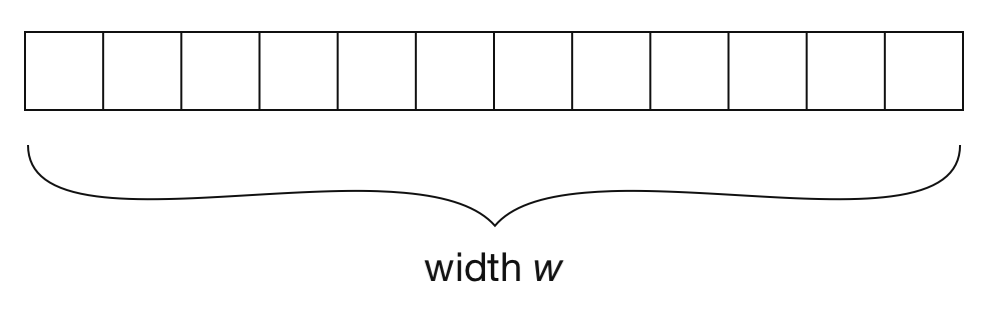
\includegraphics[width=0.5\textwidth]{figures/single_hash.png}
    \caption{Counting with a single hash}
    \label{fig:single-hash}
\end{figure}

With the help of a hash function h, we can implement a counting mechanism based on this array. To increment the count for element $x$, we hash it to get an index into the array. The cell at the respective index $h(x)$ is then incremented by 1.

Concretely, this data structure has the following operations:

\begin{itemize}
    \item Initialization: $\forall i \in \{1, \dots, w\}$: count[$i$]=0.
    \item Increment count (of element x): count[h(x)]+=1
    \item Retrieve count (of element x): count[h(x)]
\end{itemize}

This approach has the obvious drawback of hash conflicts, which result in over-counting. We would need a lot of space to make collisions unlikely enough to get accurate counts. However, we at least do not need to explicitly store keys anymore.

\textbf{More hash functions}

Instead of just using one hash function, we could use $d$ different ones. These hash functions should be pairwise independent. To update a count, we then hash item a with all $d$ hash functions, and subsequently increment all indices we got this way. In case two hash functions map to the same index, we only increment its cell once.

Unless we increase the available space, of course all this does for now is to just increase the number of hash conflicts. We will deal with that in the next section. For now let’s continue with this thought for a moment.

If we now want to retrieve a count, there are up to $d$
 different cells to look at. The natural solution is to take the minimum value of all of these. This is going to be the cell which had the fewest hash conflicts with other cells.
$$\text{min}_{i=1}^d \text{count}[\text{h}_i(x)]$$
While we are not fully there yet, this is the fundamental idea of the Count-Min Sketch. Its name stems from the process of retrieving counts by taking the minimum value.


\textbf{Fewer hash conflicts}

We added more hash functions but it is not evident whether this helps in any way. If we use the same amount of space, we definitely increase hash conflicts. In fact, this implies an undesirable property of our solution: Adding more hash functions increases potential errors in the counts.

Instead of trying to reason about how these hash functions influence each other, we can design our data structure in a better way. To this end, we use a matrix of size $w \times d$. Rather than working on an array of length $w$, we add another dimension based on the number of hash functions as shown below in fig.~\ref{fig:multi-hash}.

\begin{figure}[H]
    \centering
    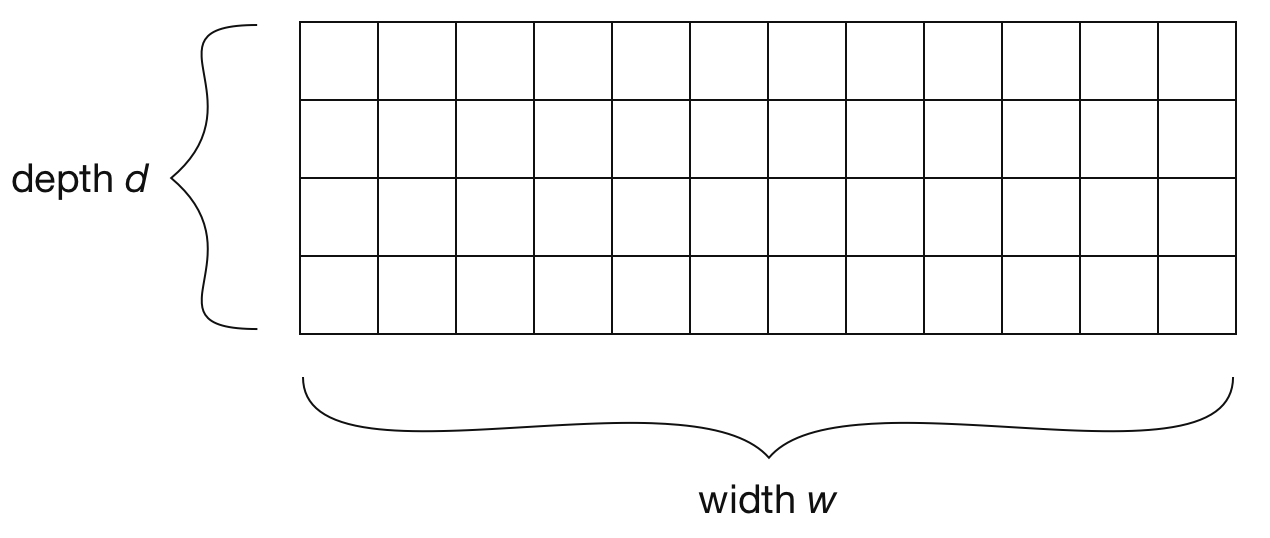
\includegraphics[width=0.5\textwidth]{figures/multiple_hashes.png}
    \caption{Counting with multiple hashes.}
    \label{fig:multi-hash}
\end{figure}

Next, we change our update logic so that each function operates on its own row. This way, hash functions cannot conflict with another anymore. To increment the count of element $a$, we now hash it with a different function once for each row. The count is then incremented in exactly one cell per row.
\begin{itemize}
    \item Initialization: $\forall i \in \{1, \dots, d\}, j \in \{1, \dots, w\}:\text{count}[i, j] = 0$ 
    \item Increment count (of element $x$):  $\forall i \in \{1, \dots, d\}:\text{count}[i,\text{h}_i(x)]$ += 1
    \item Retrieve count (of element $x$): $\text{min}_{i=1}^d \text{count}[i, \text{h}_i(x)]$
\end{itemize}


This is the full CMS data structure. We call the underlying matrix a sketch.

% stream of data items 
% q is huge
% taken from rel. large universe has exp size. Ex: this might be emails looked up in key value store
% basically estimate of the count of each of these peoople and wanna do it efficiently. 

% Explain count min sketch

\begin{subproblem}
\textbf{(10 points)} Your friend implemented the following hash functions for each row in the sketch: h$_i(x) = (x + a_i) \; \bmod \; w$ for $0 < i < d$ where $a_i$ is chosen randomly for each row, and $\bmod$ is the mod operation (sometimes written as $\%$). Is the choice of hash functions good or bad? Please justify your answer in 1 -- 2 sentences or provide a counter example.
\end{subproblem}

\begin{subproblem}
\textbf{(10 points)} Implement CMS in the function \texttt{count\_min\_sketch} in \texttt{problem\_1/p1\_b.py}. Given the vectors 
$\mathbf{a} = [a_1, \dots, a_d]$, $\mathbf{b} = [b_1, \dots, b_d]$, a scalar $p$ implement the hash function h$_i(x) = ((a_ix + b_i) \; \bmod \; p) \; \bmod \; w$. Then, use this hash function on a stream of data to create the sketch matrix.

\io The function  \texttt{count\_min\_sketch} takes in the following arguments: $\mathbf{a} = [a_1, \dots, a_d]$, $\mathbf{b} = [b_1, \dots, b_d]$ as vectors with positive entries, \texttt{w} and \texttt{p} as scalars, and a python generator function, \texttt{stream}, that produces a stream of data. The output of the function is the sketch matrix, of size $d \times w$.

\textbf{Example}

For $d=2, w=3$, given the vectors $\mathbf{a} = [1, 2]$, $\mathbf{b} = [3, 5]$, $p=100$, $w=3$, we get the following hash functions: $\text{h}_1(x) = ((x + 3) \; \% \; 100)\; \% \; 3$ , $\text{h}_2(x) = ((2x + 5) \; \% \; 100)\; \% \; 3$. For the stream of data $[10, 11, 10]$ the function \texttt{count\_min\_sketch} should return the following:\\
\texttt{[[0, 2, 1], [1, 2, 0]]} which corresponds to the following sketch matrix:
\begin{lstlisting}
0, 2, 1
1, 2, 0
\end{lstlisting}

\end{subproblem}


\end{problem}


\begin{solution}
1.(a) Please justify your answer in 1 – 2 sentences or provide a counter example.
\end{solution}

\begin{solution}
1.(b) Please submit functional code. No written component for this problem :)
\end{solution}




% \begin{problem}
% In this problem, you will design an algorithm to count the number of unique elements in a stream or database. Since the size of the given dataset is huge, it is intractable to store the entire all the elements in the stream or perform look-up on all the entries in the database. For this reason, the goal is to design a probabilistic algorithm that returns an expected number of unique elements by randomly looking at a subset of elements.
% The idea is to design an algorithm that uses a hash function to map the elements in the given dataset to a binary string, and to make use of the length of the longest null sequence in the binary string as an estimator for the number of unique elements to use as a value element. 

% \begin{subproblem}
%     Design a hashing function that hashes a given datapoint to a hash value of length 5. [TODO]
% \end{subproblem}

% \begin{subproblem}
% [TODO: I'm not entirely sure if the following will make a good problem.]
% Notice that the accuracy of the algorithm is sensitive to the distribution of entries in the sequence. 
% Consider the hash function \texttt{MyHashFunction}. 
% For this problem, you're required to design a stream of data such that  \texttt{MyHashFunction} will always produce a wrong estimate.
% \end{subproblem}

% \end{problem}

\newpage %\vspace{1cm}

\begin{problem}
% https://leetcode.com/problems/minimum-space-wasted-from-packaging/solutions/

In a charming town renowned for unique collectibles, a shopkeeper Samuel faced a challenge. He had received $n$ packages, each with distinct sizes, and needed to find boxes to match. Samuel had multiple suppliers denoted by $m$, each offering boxes of varying dimensions. His goal was to choose a supplier whose boxes would minimize the total wasted space, defined as the difference between the box and package sizes. Note that \textbf{one box can contain only one package}. Your task is to help Samuel choose a single supplier and use boxes from them such that the total wasted space is minimized. Let the size of the $i^{th}$ box be $b_i$ and the size of the $j^{th}$ package be $p_j$. For each package in a box, we define the space wasted to be $b_i - p_j$. The total wasted space is the sum of the space wasted in all the boxes.

For example, if you have to fit packages with sizes \texttt{[2,3,5]} and the supplier offers boxes of sizes \texttt{[4, 8]}, you can fit the packages of size \texttt{2} and size \texttt{3} into two boxes of size \texttt{4} and the package with size \texttt{5} into a box of size \texttt{8}. This would result in a waste of \texttt{(4-2) + (4-3) + (8-5) = 6}.


\textbf{(10 points)} Implement the function \texttt{linear\_search} in \texttt{problem\_2/p2\_a.py} that has a time-complexity of $\Theta(m \times n \times b)$ where $b$ denotes the average number of box types offered by each supplier.

\textbf{(30 points)} Implement the function \texttt{binary\_search} in \texttt{problem\_2/p2\_b.py} that has a time-complexity of $\Theta(m \times \log (n) \times b)$ where $b$ denotes the average number of box types offered by each supplier.

\io The package sizes are given as an integer array \texttt{packages}, \textbf{each with distinct sizes}, where \texttt{packages}[i] is the size of the $i^{th}$ package. The suppliers are given as 2D integer array boxes, where \texttt{boxes}[j] is an array of box sizes that the $j^{th}$ supplier produces. Return the minimum total wasted space by choosing the box supplier optimally, or -1 if it is impossible to fit all the packages inside boxes. 

\textbf{Constraints:}
\begin{flalign}
    1 \leq n \leq 10^5 \nonumber \\
    1 \leq m \leq 10^5 \nonumber \\
    1 \leq \texttt{packages}[i] \leq 10^5 \nonumber \\
    len(\texttt{boxes}[j]) \leq 10^5 \nonumber \\
    \texttt{boxes}[j][k] \leq 10^5 \nonumber  \\
    \text{The elements in } \texttt{boxes}[j] \text{ are \textbf{distinct}} \nonumber .
\end{flalign}

\textbf{Example 1:}
\begin{itemize}
    \item Input: \texttt{packages = [2,3,5]}, \texttt{boxes = [[4,8],[2,8]]}
    \item Output: 6
    \item Explanation: It is optimal to choose the first supplier, using two size-4 boxes and one size-8 box. The total waste is (4-2) + (4-3) + (8-5) = 6.
\end{itemize}

\textbf{Example 2:}
\begin{itemize}
    \item \texttt{packages = [2,3,5]}, \texttt{boxes = [[1,4],[2,3],[3,4]]}
    \item Output: -1
    \item Explanation: There is no box that the package of size 5 can fit in.
\end{itemize}


\textbf{Example 3:}
\begin{itemize}
    \item Input: \texttt{packages = [3,5,8,10,11,12]}, \texttt{boxes = [[12],[11,9],[10,5,14]]}
    \item Output: 9
    \item It is optimal to choose the third supplier, using two size-5 boxes, two size-10 boxes, and two size-14 boxes. The total waste is (5-3) + (5-5) + (10-8) + (10-10) + (14-11) + (14-12) = 9.
\end{itemize}



% \begin{lstlisting}[language=Python,caption={The adjacency dictionary representation, where the keys represent a node, and the value list represents the nodes the `key' node is connected to.},label={lst1a:codeblock},captionpos=b]
% {0:[1,3], 1:[0,2], 2:[1,3], 3:[0,2]}. 
% \end{lstlisting}

\end{problem}

\begin{solution}
    Please submit functional code. No written component for this problem :)
\end{solution}

\newpage

\begin{problem}
Dr. Carter, a scientist, is aiming to sequence a set of genes. The set is represented by a sequence of natural numbers $g_i$, where $g_i$ takes the values $1,\dots, n$,  $\forall \; i \in \{1 \dots n\}$, and where $n$ denotes the length of the sequence. Dr. Carter seeks the most efficient order to read the DNA fragments, minimizing redundancy and optimizing sequencing efforts.
Given a sequence $G = [g_1, g_2, \dots, g_n]$, there is a cost associated with processing every pair $(g_i, g_{j})$ for $1 \leq i, j \leq n$ of genes. The pairwise cost between the genes is represented as a symmetric matrix $C \in \mathbb{R}_{> 0}^{n \times n}$ where the entries in the main diagonal are set to $\infty$. Let $C(i, j)$ denote the cost associated with the pair $(g_i, g_j)$. Given a sequence of natural numbers, $s \in P(n)$, where $P(n)$ denotes the set of all permutations of the first $n$ natural numbers, let the cost associated with $s$ be denoted by $\texttt{cost}(s)$. Then $\texttt{cost}(s)$ can be computed by $$\texttt{cost}(s) = \sum_{i=1}^{n - 1} C(s_i, s_{i+1}).$$
Your job is to find an ordering $r$ that minimizes the cost associated with it .i.e.,
$$r = \textnormal{arg min}_{s \in  P(n)}\; \texttt{cost}(s).$$
Notice that this problem is NP-hard and scales poorly with increasing $n$. 



\begin{subproblem}
Since finding the optimal solution isn't tractable, one approach is to use a greedy algorithm such as the following:

\begin{lstlisting}
def greedy_solution(cost_matrix):
  n = len(cost_matrix)
  min_edge_cost = float('inf')
  min_i = None
  min_j = None
  for i in range(n):
    for j in range(n):
      if min_edge_cost > cost_matrix[i][j]:
        min_i, min_j = i, j
        min_edge_cost = cost_matrix[i][j]
  sequence = [min_i, min_j]
  r = min_j
  for _ in range(n - 1):
    min_entry = float('inf')
    min_col = None
    for j in range(n):
      if min_entry > cost_matrix[r][j]:
        min_entry = cost_matrix[r][j]
        min_col = j
    sequence.append(min_col)
    r = min_col
  return sequence
\end{lstlisting}

This function can be found in \texttt{problem\_3/p3\_a.py} file. The solution found by this greedy approach is a sub-optimal solution. Design a cost matrix for $n=4$ such that the solution predicted by the greedy algorithm corresponds to the worst solution i.e. the sequence with the highest cost. %\carolina{I think it is a bit confusing why we talk about the 4x4 matrix here and then repeated in the next paragraph, but no strong feelings about it }
\end{subproblem}

\textbf{(20 points)} You are required to design the cost matrix $C$, which is a matrix of size $4 \times 4$. The matrix should be put in \texttt{problem\_3/p3\_a.txt}. The objective is to structure the cost matrix in a manner that ensures the solution returned by \texttt{greedy\_solution} in \texttt{problem\_3/p3\_a.py} has the maximum cost compared to all other potential solutions.

\io The cost matrix, described as a $4 \times 4$ matrix with positive entries, can be represented in a text file named \texttt{p3\_a.txt} in the following format:

\begin{lstlisting}
inf, 1, 2, 3
4, inf, 6, 7
5, 9, inf, 11
12, 13, 14, inf
\end{lstlisting}

In this representation:
\begin{itemize}
    \item Each line in the file corresponds to a row in the cost matrix.
    \item The entries in each row are comma-separated, representing the values in the respective columns of the cost matrix.
    \item The symbol \texttt{inf} represents infinity.
\end{itemize}


\begin{subproblem}
Now we'll use a local search method to improve upon the greedy approach. Given a candidate solution, the idea is to iteratively improve the solution by making ``small'' changes to it. The algorithm is outlined as follows:

\begin{enumerate}
    \item Initialization: Start with an initial candidate sequence with a random ordering of entries.
    \item Neighbor Generation: Choose two genes in the candidate. Consider swapping the genes, creating a new ``potential'' solution for the next iteration.
    \item Evaluate the cost associated with the change: Calculate the change in cost resulting from the swap. If the ``potential'' candidate has a smaller cost than the current candidate, accept the change. Otherwise, maintain the current candidate.
    \item Iterate: Repeat steps 2-3 for all possible pairs of genes in the candidate. This constitutes one iteration.
    \item Termination:
    Run multiple iterations, i.e. step 4, until no more improvements can be made.
\end{enumerate}
\end{subproblem}

\textbf{(20 points)} Implement the function \texttt{local\_search\_2opt} in \texttt{problem\_3/p3\_b.py}.

\io The cost matrix, \texttt{c}, is given as a $n \times n$ matrix with positive entries, the candidate solution, \texttt{init}, is given as a random permutation of the natural numbers $[1, \dots, n]$. Return the updated solution by repeatedly applying 2-opt as outlined above. 

\textbf{Example:}
\begin{itemize}
    \item \texttt{c = [[inf, 3, 5], [3, inf, 7], [5, 7, inf]]}, \texttt{candidate = [2, 3, 1]}
    \item Output: \texttt{candidate = [2, 1, 3]}
    \item Explanation: The cost of the candidate solution, denoted as \texttt{candidate = [2, 3, 1]}, is calculated as $\texttt{C}(2, 3) + \texttt{C}(3, 1) = 7 + 5 = 12$. The neighboring candidates, namely \texttt{[3, 2, 1]} and \texttt{[2, 1, 3]}, have costs of $10$ and $8$, respectively. Therefore, after the first iteration, the new candidate becomes \texttt{[2, 1, 3]}.
    Moving to the next iteration, the candidate \texttt{[2, 1, 3]} has neighbors \texttt{[1, 2, 3]} and \texttt{[2, 3, 1]}, with costs of $10$ and $12$, respectively. Since the neighboring solutions have higher costs, the candidate solution remains unchanged, and the algorithm converges. Consequently, the final solution is \texttt{[2, 1, 3]}.
\end{itemize}
\end{problem}


\begin{solution}
    Please submit functional code. No written component for this problem :)
\end{solution}

\newpage


%%%%%%%%%%%%%%%%%%%%%%%%%%%%%%%%%%%%%%%%%%%%%%%%%%%%%%%%%%%%%%%%%%%%%%%%%%%%%%%%
% Challenge
 \begin{challenge}
% https://leetcode.com/problems/ones-and-zeroes/description/

Once upon a time in the digital kingdom, there existed an array of binary strings known as \texttt{strs}. These strings, comprising only of 0s and 1s, held the secrets to unlocking great possibilities. Alongside these mysterious strings, two wise integers named \texttt{m} and \texttt{n} entered the scene, bearing a quest for knowledge.

The mission presented to the inhabitants of the digital realm was to uncover the size of the largest subset within the array of binary strings. However, this was no ordinary quest. The conditions were set by the integers \texttt{m} and \texttt{n} - they imposed limits on the number of 0s and 1s that the chosen subset could possess.

The quest's rules were clear: the subset's size must be maximized, but within the constraints of having at most \texttt{m} 0s and \texttt{n} 1s. A set \texttt{x} was considered a subset of another set \texttt{y} only if every element in \texttt{x} was also present in \texttt{y}.

% You are given an array of binary strings \texttt{strs} and two integers \texttt{m} and \texttt{n}.
% Return the size of the largest subset of \texttt{strs} such that there are at most \texttt{m} 0's and \texttt{n} 1's in the subset. A set \texttt{x} is a subset of a set \texttt{y} if all elements of \texttt{x} are also elements of \texttt{y}.

Implement the function \texttt{find\_max\_form} in \texttt{challenge/challenge.py}.

\io \texttt{strs} is given as an array of binary strings, \texttt{m} and \texttt{n} are integers. Return an integer that represents the size of the largest subset of \texttt{strs} with at most m 0's and n 1's. 

\textbf{Example 1:}
\begin{itemize}
    \item Input: \texttt{strs = ["10", "0001", "111001", "1", "0"]}, \texttt{m = 5, n = 3}
    \item Output: 4
    \item The largest subset with at most 5 0's and 3 1's is \texttt{\{"10", "0001", "1", "0"\}}, so the answer is 4. Other valid but smaller subsets include \texttt{\{"0001", "1"\}} and \texttt{\{"10", "1", "0"\}}. \texttt{\{"111001"\}} is an invalid subset because it contains 4 1's, greater than the maximum of 3.
\end{itemize}

\textbf{Example 2:}
\begin{itemize}
    \item Input: \texttt{strs = ["10","0","1"]}, \texttt{m = 1, n = 1}
    \item Output: 2
    \item The largest subset is \texttt{\{"0", "1"\}}, so the answer is 2.
\end{itemize}


\end{challenge}


\begin{solution}
    Please submit functional code. No written component for this problem :)
\end{solution}

\end{document}